\documentclass[conference]{IEEEtran}
\usepackage[utf8]{inputenc}
\usepackage[T1]{fontenc}
\usepackage[final]{pdfpages}
\usepackage[french]{babel}
\usepackage{colortbl}
\usepackage[table]{xcolor}
\usepackage{verbatim} 
\usepackage{graphicx}
\usepackage{algorithmicx}
\usepackage{algorithm}
\usepackage{cite}
\usepackage{amsmath}
\newtheorem{theo}{Propriété} 
\usepackage[caption=false,font=footnotesize]{subfig}
\usepackage[left = 3.5cm, right = 3.5cm, top = 4cm, bottom = 4cm]{geometry}

\usepackage{fancyhdr}

\title{Vérification des propriétés de sûreté d'un protocole de loterie Bitcoin}
\author{\IEEEauthorblockN{Guillaume Stunault}
\IEEEauthorblockA{Etudiant \\ Telecom Nancy}
\and \IEEEauthorblockN{Lucas Vignali} 
\IEEEauthorblockA{Etudiant \\ Telecom Nancy} }


\date{\today}

\begin{document}

\maketitle
\begin{abstract}
Les Smart Contracts sont des programmes qui exécutent de façon automatique les termes d'un contrat, et sans besoin d'une tierce-personne de confiance pour vérifier leur bon déroulement\cite{ethercontract}.
Ils sont de plus en plus utilisés avec l'essor de la blockchain et des cryptomonnaies. Ainsi leur sécurité et leur exactitude sont cruciales pour garantir l'équité entre les différentes parties\cite{bcfr-smart, smartdeloitte}.
Nous nous sommes donc intéressés à un protocole de loterie Bitcoin \cite{955} afin de vérifier plusieurs de ces propriétés de sécurité avec Tamarin\cite{tamarin}.
\end{abstract}
\section{Introduction}

Pour notre projet de PIDR nous avions comme sujet : \textbf{Vérification des « smart contracts » sur la blockchain}. Ce sujet nous a été proposé par M. Jannik DREIER, membre du LORIA et de l'équipe PESTO, accompagné de M. Steve Kremer. \\Suite à l'essor des applications liées à la blockchain et principalement celle du Bitcoin, les "Smart Contracts" se sont développés. Comme l'exécution du "Smart contract" est automatique, il est nécessaire de s'assurer de la sécurité de ces protocoles afin qu'aucun participant ne soit lésé durant l'exécution. Par exemple, pour une loterie, il faut s'assurer qu'aucun participant ayant signé le contrat puisse gagner sans avoir misé.

Le but de ce PIDR a donc été de modéliser un système de smart contract. Pour cela nous avons utilisé un logiciel créé par l'équipe PESTO du LORIA : \textbf{Tamarin}\cite{tamarin}. Sur ce logiciel nous avons modélisé un protocole de loterie et vérifié certaines \textbf{propriétés de sûreté} (qu'une exécution incorrecte est impossible).
\newpage
\section{État de l'art}
\subsection{La Blockchain}
La blockchain est une technologie de stockage et de transmission d’informations, transparente, sécurisée, et fonctionnant sans organe central de contrôle.

Une blockchain constitue une base de données qui contient l’historique de tous les échanges effectués entre ses utilisateurs depuis sa création. Ces échanges sont enregistrés sous forme de blocs, qui mis bout à bout forment une chaîne, d'où le terme blockchain. \\Cette base de données est sécurisée et distribuée : elle est partagée par ses différents utilisateurs, sans intermédiaire, ce qui permet à chacun de vérifier la validité de la chaîne \cite{bcfr}.

\begin{figure}[!h]
    \centering
    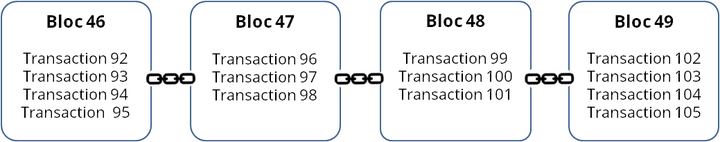
\includegraphics[scale=0.55]{blck-schema.png}
    \caption{\textit{Représentation d'une blockchain \cite{bcfr}}}
    \label{fig:blockchain}
\end{figure}
\vspace{0.2cm}

L’intérêt de la blockchain réside dans l’aspect décentralisé de la base de données qui est stockée sur les différents serveurs des utilisateurs et fonctionne sans intermédiaire ce qui limite les frais d’infrastructure. Cette base de données que beaucoup comparent à un grand livre comptable – public et partagé – contient un historique infalsifiable des transactions qui est mis à jour en temps réel par les utilisateurs. Les utilisateurs valident chaque transaction et vérifient la cohérence de celle-ci grâce au registre. \\

\textbf{Pourquoi infalsifiable ? } \\
Distribuée, et non centralisée, la base de données est aussi doublement sécurisée. D'abord par un système de cryptographie dite "asymétrique". En effet, pour soumettre une transaction dans la blockchain, le mandataire doit auparavant la signer avec sa clé privée.

Ensuite, chaque bloc est validé par les noeuds du réseau appelés les “mineurs”. Les "mineurs" chargés de vérifier la validité des transactions bloc par bloc sont des particuliers, rémunérés pour mettre à disposition la puissance de calcul de leurs processeurs en résolvant des fonctions de hachage cryptographique afin de chiffrer l'ensemble des transactions d'un bloc ainsi que les transactions chiffrées de la chaîne de bloc précédente. \\Cette technique s'appelle le "Proof-of-Work" (preuve de travail), c'est la méthode utilisée dans la blockchain Bitcoin\cite{7x7, PoW}. \\

Comme chaque bloc contient le hachage du bloc précédent, corrompre un bloc va revenir à créer une branche valide à partir du bloc corrompu. 
Si un pirate souhaite corrompre un bloc, il va devoir créer une chaîne de blocs valide à partir de ce bloc modifié. S'il souhaite que sa chaîne de bloc soit considérée valide par l'ensemble du réseau, il faut qu'elle soit plus longue que la chaîne principale constituée des blocs ajoutés par les mineurs à partir du bloc non corrompu.\\
Ainsi pour manipuler la blockchain, il faudrait pouvoir falsifier plus de la moitié de la puissance de calcul du système, ce qui est techniquement difficile, voire impossible à réaliser. \vspace{0.15cm}

\begin{figure}[!h]
    \centering
    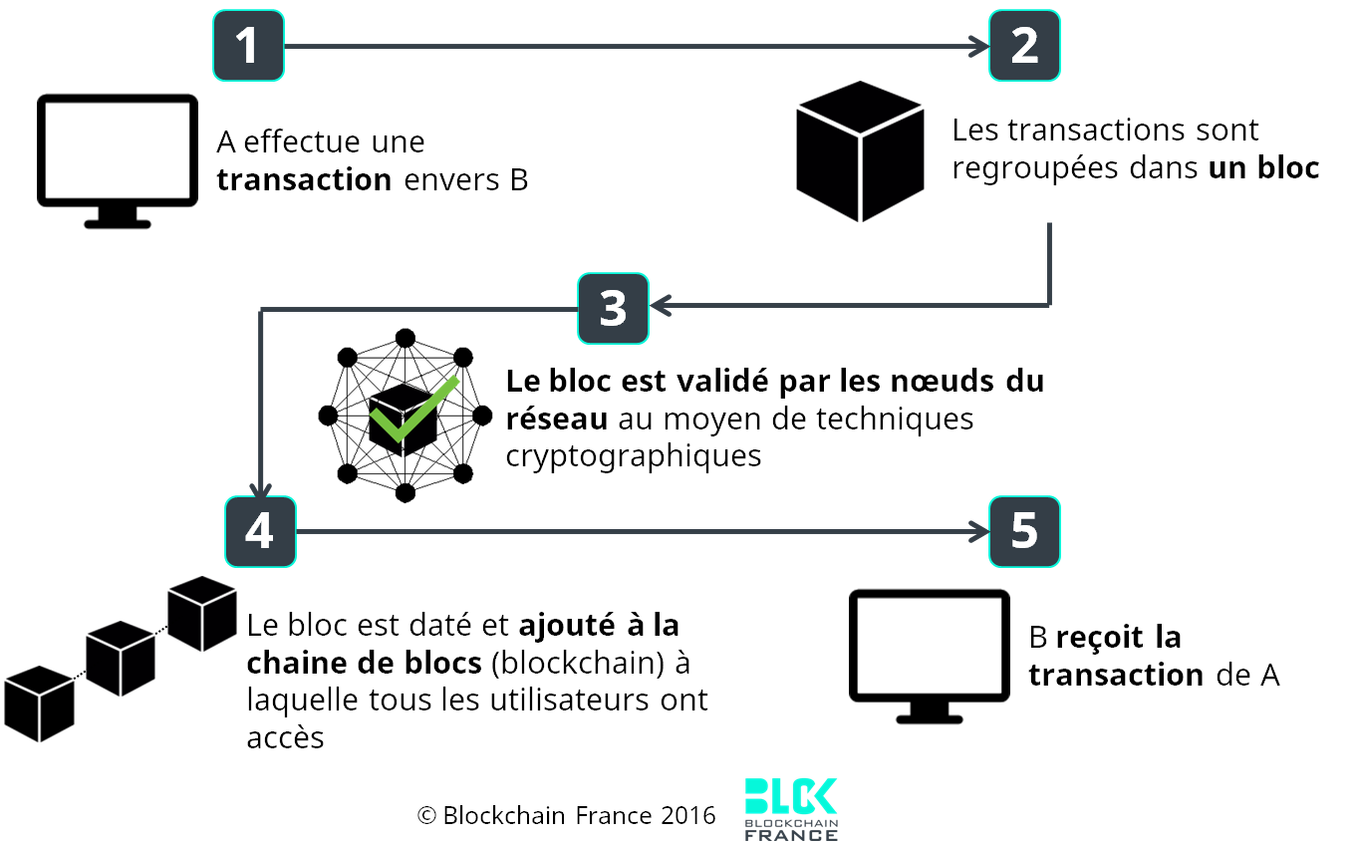
\includegraphics[scale=0.3]{blck-fonctionnement.png}
    \caption{\textit{Fonctionnement de la blockchain} \cite{bcfr}}
    \label{fig:blck-fonctionnement}
\end{figure}
\vspace{0.3cm}\\

\newpage

\textbf{Le potentiel de la blockchain} \cite{bcfr}\\

Bien que souvent associée au Bitcoin et autres cryptomonnaies, le caractère décentralisé de la blockchain, couplé avec sa sécurité et sa transparence, promet des applications bien plus larges : 
\begin{itemize}
    \item Les applications pour le transfert d’actifs (utilisation monétaire, mais pas uniquement : titres, votes, actions, obligations…)
    \item Les applications de la blockchain en tant que registre : elle assure ainsi une meilleure traçabilité des produits et des actifs.
    \item Les smart contracts : il s’agit de programmes autonomes qui exécutent automatiquement les conditions et termes d’un contrat, sans nécessiter d’intervention humaine une fois démarrés. 
\end{itemize} 


\subsection{Le Bitcoin}

Le Bitcoin est une monnaie virtuelle mais aussi un système de paiement pair à pair. C'est la première monnaie électronique décentralisée. Ce type de monnaie possède différents avantages : 
\begin{itemize}
    \item Échange de particulier à particulier ce qui implique des frais inférieurs à ceux des banques
    \item Utilisable dans tous les pays
    \item Les comptes ne peuvent pas être gelés
    \item Anonymat des transactions
\end{itemize}
\vspace{0.3cm}

Les bitcoins peuvent être générés par toute personne possédant un ordinateur et faisant tourner un logiciel appelé "mineur de bitcoin". \\Cette création de bitcoin requiert de travailler sur chaque bloc de transaction. Ceci est ajusté par le réseau pour que la création des bitcoins soit prédictible et limitée. Enfin les bitcoins sont stockés dans des porte-monnaie électroniques. Chaque transaction est vérifiée puis stockée sur le réseau.

\vspace{0.3cm}

\subsection{Les smart contracts}
Les \textbf{smarts contracts} sont des programmes autonomes qui une fois lancés exécutent automatiquement des conditions définies préalablement et inscrites sur la blockchain. Par exemple c'est ce qu'il se passe lorsque l'on souscrit à une assurance et que en cas de problème on est remboursé sans avoir à faire quelque chose.
L'avantage de ce type de contrat repose sur le fait qu'ils sont dans la blockchain, et donc qu'ils ne sont pas modifiables. Dans le cas où ils ne seraient pas dans la blockchain, alors ils seraient modifiables.

\vspace{0.3cm}
\subsection{Notions cryptographiques nécessaires à la compréhension du protocole}

\subsubsection{Cryptographie asymétrique}
Le principe de chiffrement asymétrique (appelé aussi chiffrement à clés publiques) est apparu en 1976, avec la publication d'un ouvrage sur la cryptographie par Whitfield Diffie et Martin Hellman\cite{ccmasym, clepub}. 


Dans un cryptosystème asymétrique (ou cryptosystème à clés publiques), les clés existent par paires (le terme de bi-clés est généralement employé) :
\begin{itemize}
    \item Une clé publique pour le chiffrement
     \item Une clé secrète pour le déchiffrement
\end{itemize}
    
Ainsi, dans un système de chiffrement à clé publique, les utilisateurs choisissent une clé aléatoire qu'ils sont seuls à connaître (il s'agit de la clé privée). A partir de cette clé, ils déduisent chacun automatiquement une clé publique. Les utilisateurs peuvent s'échanger cette clé publique au travers d'un canal non sécurisé.

Lorsqu'un utilisateur désire envoyer un message à un autre utilisateur, il lui suffit de chiffrer le message à envoyer au moyen de la clé publique du destinataire. Ce dernier sera en mesure de déchiffrer le message à l'aide de sa clé privée (qu'il est le seul à connaître)\cite{ccmasym}. 

\begin{figure}[!h]
    \centering
    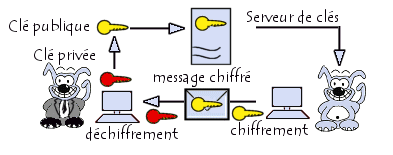
\includegraphics[scale=0.7]{asym.PNG}
    \caption{\textit{Envoi de messages par chiffrement asymétrique} \cite{ccmasym}}
    \label{fig:asym}
\end{figure}

Ce chiffrement permet de s'assurer que \textbf{seul le destinataire du message peut le déchiffrer}. \\
Certaines signatures, comme \textbf{RSA}, utilisent le chiffrement asymétrique pour chiffrer le message.

\vspace{0.3cm}
\subsubsection{Les fonctions de hachage cryptographique}
Une fonction de hachage cryptographique est une fonction qui, à une donnée de taille arbitraire, associe une image de taille fixe. \\Une propriété essentielle est qu'elle est pratiquement impossible à inverser, c'est-à-dire que si l'image d'une donnée par la fonction se calcule très efficacement, le calcul inverse d'une donnée d'entrée ayant pour image une certaine valeur se révèle impossible sur le plan pratique. Pour cette raison, on dit d'une telle fonction qu'elle est à sens unique\cite{wikihash, ryxhash}.

Les fonctions de hachage sont utilisées pour garantir \textbf{l'intégrité} d'une donnée. Si un message est corrompu, son haché ne sera plus le même\cite{igmsign}. \\
Une fonction de hachage transforme un message de taille arbitraire en message de taille fixe. Il y a donc un problème : comme il y a plus de messages possibles que de hachés possibles, plusieurs messages peuvent donc avoir le même haché. Cela s'appelle une collision\cite{ryxhash, cryptohash}. \\
Pour une fonction de hachage F, on demande qu'elle soit :
\begin{itemize}
    \item résistante au calcul de préimage (étant donné y difficile de trouver y = F(x))
    \item résistante au calcul de seconde préimage (étant donné x, difficile de trouver x', tel que F(x) = F(x'))
    \item résistante aux collisions (difficile de trouver x et x', tel que F(x) = F(x'))
\end{itemize}
\vspace{0.2cm}
Il est aujourd'hui très difficile de trouver des collisions sur les fonctions de hachage actuelles (SHA2-SHA3). \\
Les fonctions de hachage modélisées dans Tamarin sont résistantes aux 3 propriétés ci-dessus. \\


\subsubsection{Signature}
La signature d'un document permet de garantir l'identité du signataire. 5 caractéristiques sont nécessaire pour définir une signature \cite{igmsign}:

\begin{itemize}
    \item \textbf{authentique} (on est certain de l'identité du signataire)
    \item \textbf{infalsifiable}
    \item \textbf{non réutilisable} (la signature est unique au document)
    \item \textbf{inaltérable} (un document signé ne peut plus être modifié)
    \item \textbf{irrévocable} (une personne ne peut pas nier avoir signé un document)
\end{itemize}

\vspace{0.3cm}
Une architecture de signature possible peut être obtenue en combinant le chiffrement asymétrique et les fonctions de hachage.

Si Alice souhaite signer un document et l'envoyer à Bob : \\
    Tout d'abord, elle génére \textbf{l'empreinte} du document au moyen d'une fonction de hachage.\\
    Puis, elle crypte cette empreinte avec sa clé privée.

    Elle obtient ainsi la signature de son document. Elle envoie donc ces deux éléments à Bob

    Pour vérifier la validité du document, Bob doit tout d'abord déchiffrer la signature en utilisant la clé publique d'Alice. Si cela ne fonctionne pas, c'est que le document n'a pas été envoyé par Alice.\\
    Ensuite, Bob génère l'empreinte du document qu'il a reçu, en utilisant la même fonction de hachage qu'Alice (On supposera qu'ils suivent un protocole établi au préalable).\\
    Puis, il compare l'empreinte générée et celle issue de la signature.

    Si les deux empreintes sont identiques, la signature est validée. Pour cette architecture de signgature qui utilise le chiffrement asymétrique, nous sommes donc sûr que : \\
        C'est Alice qui a envoyé le document, \\
        Le document n'a pas été modifié depuis qu'Alice l'a signé \cite{igmsign}.


La signature numérique garantit \textbf{l'identité} du signataire et \textbf{la non répudiation} du document signé par le signataire.

Dans Tamarin, il existe plusieurs fonctions qui utilisent la signature :
\begin{itemize}
    \item sign : Cette fonction permet de signer un message à partir d'une clé secrète
    \item verifySign : Cette fonction permet de vérifier l'identité du signataire du message à partir de sa clé publique
    \item revealingSign : Cette fonction permet de retirer la signature d'un message à partir de la clé secrète du signataire
\end{itemize}
\subsection{Tamarin}

Tamarin est un logiciel collaboratif pour l'analyse symbolique et l'analyse de protocoles de sécurité. Ce logiciel permet donc de modéliser des protocoles pour vérifier leur exécution. L'écriture de protocole dans ce logiciel se décompose en plusieurs étapes. Tout d'abord on peut utiliser des fonctions déjà existantes par l'intermédiaire de built-in fonctions ~\ref{B-I}. Ces built-in permettent par exemple de modéliser des fonctions de hachage. \\

\begin{center}
\begin{figure}[!h]
\centering
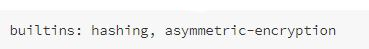
\includegraphics[scale=0.6]{BuiltIn.JPG}
\caption{Built-In Tamarin qui contiennent des fonctions pré-définies}
\label{B-I}
\end{figure}
\end{center}

Ensuite il faut créer les règles. Les règles opèrent sur l'état du système exprimé sous la forme d'un multi-ensemble de \textbf{faits}. Les faits sont en fait des prédicats contenant les informations d'états. Une fois toutes les règles, décrivant le fonctionnement du protocole, écrites on peut passer à l'écriture des propriétés. \\ 
En effet, il faut ensuite écrire les propriétés permettant de vérifier la bonne exécution du protocole. Pour cela il faut trouver et écrire des propriétés de sécurité principalement. Par exemple nous avons écrit une propriété vérifiant que la somme de Bitcoin en jeu dans notre protocole est constante, il n'y a pas d'argent ajouté ou perdu au cours d'une partie. Par exemple pour la propriété décrite ci-dessus, il faut regarder sur chaque trace du protocole si la somme des porte-monnaie des joueurs est bien égale à la totalité des gains mis en jeu au départ. Nous avons au final 5 lemmes détaillés dans la partie \ref{sec:sec-5}. \\


\subsubsection{Création d'une règle} 
Pour créer une règle il faut tout d'abord lui donner un nom, elle se déclare tout simplement par : \textbf{rule Nom\_Règle}. Ensuite, une règle contient 3 parties : 
\begin{itemize}
    \item Les entrées
    \item Les sorties
    \item Les "actions facts" \\
\end{itemize}

Les entrées correspondent tout simplement aux conditions d'entrée. Si on a cette entrée alors on applique la règle. La sortie détermine ce qui ressort de la règle. Enfin il y a les "actions facts", ils ressemblent aux faits mais contrairement à eux ils n'apparaissent que sur la trace. Ce sont les "actions facts" qui permettent de vérifier les lemmes. \\
Finalement une règle s'écrit sous la forme : \\
\textbf{rule Nom\_Règle : }\\
\textbf{ [ Entrées ]}\\
\textbf{ --[Action facts]->}\\
\textbf{ [ Sorties ]}\\

\subsubsection{Création d'un lemme} 
Les lemmes, ou propriétés, servent à vérifier la bonne exécution du protocole.\\
Pour vérifier la propriété dans Tamarin, il faut parcourir les traces lors de l'exécution. Par exemple on peut regarder si à la fin on a bien un gagnant. Un lemme s'écrit de cette manière :\\
\textbf{lemme Nom\_Lemme : }\\
\textbf{exists-trace}\\
\textbf{" Ex J #i. Win(J) @ i "}

\newpage

\section{Le protocole de loterie}
Nous allons analyser ce protocole de smart contract qui implémente une loterie Bitcoin\cite{955}. 
Ce protocole garantit :
\begin{itemize}
\item chaque joueur honnête aura (en moyenne) un gain non négatif, même dans la
présence d'adversaires qui jouent contre 
\item Si tous les joueurs sont honnêtes, le protocole simule une loterie ordinaire : 1 joueur remporte les mises des autres joueurs 
\end{itemize}
Le protocole utilise un arbre de tournoi : chaque manche le gagnant remporte la mise de l'adversaire \\
\begin{figure}[!h]
    \centering
    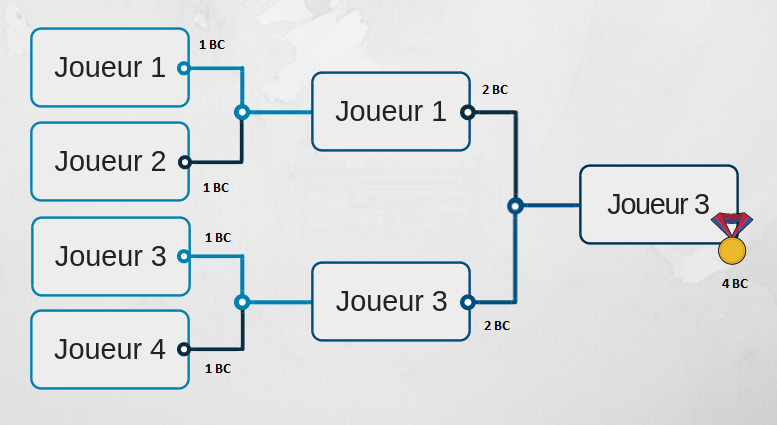
\includegraphics[scale=0.35]{arbre-tournoi.png}
    \caption{\textit{Protocole pour 4 joueurs avec mise de départ : 1 Bitcoin}}
    \label{fig:my_label}
\end{figure}
\vspace{0.3cm}\\
Initialisation : \\
\begin{itemize}
\item chaque joueur génère N paires de clés, O(N\up{2}) signatures (N signatures pour N paires de clé * N transactions Win, Timeout... pour chaque joueur) et log(N) secrets qu'il hash ensuite pour tous les matchs qu'il va jouer.
\item on vérifie que les hashs ne sont pas réutilisés
\item ensuite il pose la mise en signant une transaction Init
\item si un joueur ne pose pas la mise, les autres récupèrent leur mise
\item Init est ajouté à la blockchain
\item La transaction doit s'effectuer dans un temps donné, assez long pour qu'il permette la transaction. Ce temps est calculé pour permettre la géneration des clés 
\item Init est ensuite séparée en N mises de départ : Win(p,p) ajoutées à la blockchain \\
\end{itemize}



Execution :  \\
\begin{itemize}
\item C'est la phase de match, soient $\pi_{k}$ le nombre de duels restants, $p_{1}$ et $p_{2}$ les joueurs qui s'affrontent
\item Au départ, on ajoute à la blockchain, les transactions Win( $\pi_{k-1}$, $p_{1}$) et Win( $\pi_{k-1}$, $p_{2}$) si ça n'a pas déjà été fait
\item $p_{1}$ commence, on ajoute Turn1($\pi_{k}$, $p_{1}$, $p_{2}$) à la blockchain :  $p_{1}$ doit donc révéler son secret à temps en l'ajoutant, comme entrée dans Turn2($\pi_{k}$, $p_{1}$, $p_{2}$)
\item Ainsi, $p_{2}$ peut vérifier que le hash de $p_{1}$ correspond au hash envoyé au départ
\item $p_{2}$ envoie également son propre secret dans le temps imparti
\item La blockchain exécute alors la fonction aléatoire w = winner($\pi_{k}$, $p_{1}$, $p_{2}$, $Sk_{1}$, $Sk_{2}$) qui permet de désigner le gagnant selon la parité des secrets. Ensuite la blockchain peut ajouter la transaction Win(w, $\pi_{k}$) qui signifie que w a gagné la manche et qu'il peut participer au tour suivant.
\item Chaque joueur doit chacun son tour révéler sa clé dans un temps imparti sinon il perd. \\
\end{itemize}\\

Fin :\\
A la fin de l'exécution, $\pi_{k}$ vaut 0, le gagnant est w dans la dernière transaction Win(w, 0). La blockchain ajoute alors ensuite une transaction bitcoin vers le porte-monnaie de w (clé publique de w) qui contient le montant de la loterie.\\

Mise : \\
 A tous les tours, chaque joueur mise 1 bitcoin. Pour éviter la fraude et qu'un joueur quitte la partie en plein milieu avec l'argent qu'il a récolté, chaque joueur pose au début une somme de bitcoins égale au nombre de parties possibles par un joueur. Ainsi à chaque partie gagné un bitcoin est retiré de cette somme, et si le joueur quitte la partie en plein milieu cette est reversé à chaque joueur affronté précédemment ce qui fait que le joueur en question ne gagne pas d'argent. Dans le cas où il perd une manche cette mise lui est rendu.

\section{Protocole réalisé}
Nous avons simplifié le protocole au maximum pour tester ses diverses propriétés de sécurité. \\

Nous prenons désormais uniquement \textbf{2 joueurs} A et B, et une seule manche de match. \\
La mise vaut pour le moment : \textbf{1 bitcoin} \\
Nous définissons en brut la somme que contient les porte-monnaie des 2 joueurs (\textbf{3 bitcoins}). \\

De plus, nous nous sommes servis \textbf{des traces} de Tamarin pour modéliser une blockchain. En effet, les traces de Tamarin forment un historique et sont consultables à chaque moment, tout comme les transactions enregistrées sur la blockchain.

Ainsi, durant l'exécution de ce protocole, nous utilisons Tamarin pour \textbf{modéliser} la \textbf{blockchain}. \\


\begin{itemize}
    \item A et B génèrent chacun une clé publique et une clé secrète
    \item A partir de cette clé secrète, le protocole assigne un porte-monnaie avec 3 bitcoins à chaque joueur
    \item Chacun des 2 joueurs génère ensuite un secret pour le match, et envoie son hash signé sur le réseau.
    \item La blockchain retire 1 Bitcoin du porte-monnaie de A et B pour créer une mise
    \item La blockchain crée un contrat où A et B posent leurs mises. Lorsque les 2 mises sont posées, le match peut commencer.
    \item La blockchain crée un contrat où A doit révéler son secret. Elle vérifie que le hash du secret envoyé correspond au hash envoyé avant le match
    \item Idem pour B
    \item Lorsque la blockchain possède les 2 hashs, elle peut déterminer aléatoirement un gagnant entre A et B.
    \item La blockchain ajoute les 2 Bitcoins au porte-monnaie du gagnant.
\end{itemize}
\vspace{0.2cm}
Normalement, la blockchain est censée déterminer un gagnant avec une fonction sur la parité des secrets (processus qui est défini aléatoire et non trucable). \\Pour modéliser cela sur Tamarin, nous avons créé 2 règles identiques de victoire : une avec A, une avec B. Tamarin choisit alors aléatoirement de manière disjointe une de ces 2 règles.\\

On identifie chaque joueur de façon unique dans les traces du protocole par sa \textbf{clé secrète}. Cela permet de s'assurer que le joueur qui joue et qui peut remporter la mise, est l'un des joueurs qui a déposé l'argent.\\
Voilà les règles que nous avons créés dans Tamarin : 
\begin{itemize}
    \item CreerPK : Cette règle permet à chaque joueur de créer une clé publique et une clé secrète.
    \item CreerSecret : Cette règle permet à un joueur de créer un secret, et de l'envoyer signé sur le réseau.
    \item LArgent : Cette règle retire à chaque joueur la mise. Le joueur signe ensuite sa mise, et l'envoie sur le réseau.
    \item Init : Lorsque le protocole a reçu toutes les signatures (ici uniquement 2), il crée une règle MatchA entre ces 2 joueurs.
    \item MatchA : Cela signifie que c'est au tour de A de révéler son secret. La blockchain vérifie que le secret que A révèle est bien celui qu'il a signé et envoyé sur le réseau. Ensuite, une règle MatchAB est créée.
    \item MatchAB : C'est au tour de B de révéler son secret. La blockchain effectue la même vérification que pour A. Ensuite, la blockchain crée aléatoirement, une règle WinnerA ou WinnerB.
    \item WinnerA/WinnerB : Le joueur récupère dans son porte-monnaie la mise en jeu.
\end{itemize}
\vspace{0.3cm}

Ainsi, contrairement au protocole original \cite{955} qui prend en compte le temps passé. C'est à dire, que si un joueur ne joue pas ou reste bloqué trop longtemps dans une règle, alors il est considéré \textbf{perdant}. Notre protocole sur Tamarin peut rester bloqué indéfiniment dans une règle si le joueur refuse de jouer.

En effet, gérer le temps dans Tamarin est assez compliqué à réaliser, et nous n'avons pas eu le temps de le faire. 

\section{Propriétés à prouver}
\label{sec:sec-5}
Nous avons décidé, pour vérifier le bon fonctionnement du protocole d'implémenter des propriétés simples. Nous avons donc modélisé 3 propriétés :
\begin{itemize}
    \item Il existe une exécution normale du protocole
    \item A la fin, le porte-monnaie du gagnant contient 4 bitcoins, et celui du perdant 2 bitcoins
    \item Il y a un seul gagnant à la fin, qui peut être le joueur A ou le joueur B \\
\end{itemize}
Ces propriétés étaient en partie formulées dans la documentation du protocole.
Chaque preuve de ses propriétés se décrit sous forme de lemme. Par exemple pour vérifier que le joueur A ou le joueur B peut gagner il faut regarder s'il existe une version de l'exécution (trace) du protocole où à la fin on a WinnerA ou WinnerB (les fonctions définissant le gagnant).\\

Pour montrer que Tamarin est capable de désigner A ou B comme gagnant, on va montrer qu'il existe bien au moins une trace où A gagne, et une où B gagne : 
\begin{figure}[!h]
    \centering
    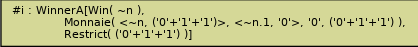
\includegraphics[scale=0.62]{winnerA.png}
    \caption{\textit{Dernière règle de la trace où A remporte le match}}
    \label{fig:winnerA}
\end{figure}
\vspace{-0.3cm}
\begin{figure}[!h]
    \centering
    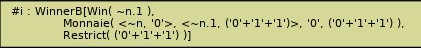
\includegraphics[scale=0.62]{winnerB.png}
    \caption{\textit{Dernière règle de la trace où B remporte le match}}
    \label{fig:winnerB}
\end{figure}


A possède la clé secrète ~n, B possède la clé secrète ~n.1. \\On remarque bien que les 2 règles WinnerA et WinnerB sont utilisées. \\Et que c'est bien A qui gagne le match dans WinnerA et B qui gagne dans WinnerB. 

\vspace{0.2cm}
Nous avons également choisi de prouver des propriétés qui s'appliquent pour toutes les traces de l'exécution.
\vspace{0.3cm}\\

\textbf{Un seul gagnant} 

On cherche à montrer que 2 joueurs ne peuvent pas gagner en même temps. \\
Pour cela, nous avons ajouté un fait Win(sk) qui contient la clé secrète du gagnant dans chacune des règles WinnerA/WinnerB.
\vspace{0.2cm}
\begin{theo}
\textbf{All skA skB #i #j. Win(skA)@i & Win(skB)@j & not(skA=skB) ==> F}
\end{theo}
\vspace{0.3cm}
Cela signifie que si on se limite à une exécution du protocole : c'est impossible d'avoir 2 clés secrètes skA, skB différentes, et 2 faits Win(skA) au moment i, Win(skB) au moment j.



\begin{figure}[!h]
    \centering
    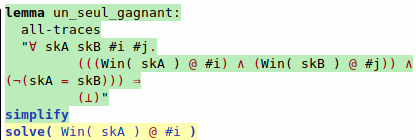
\includegraphics[scale=0.62]{ungagnant.png}
    \caption{\textit{Propriété un\_seul\_gagnant prouvée par Tamarin}}
    \label{fig:my_label}
\end{figure}\\


\textbf{Répartition correcte de l'argent sur chaque trace} 

Pour vérifier que la somme d'argent en jeu est juste pendant toute l'exécution du contrat, nous avons ajouté un fait Monnaie qui contient le porte-monnaie du joueur A, le porte-monnaie du joueur B, la somme mise en jeu et le total : Monnaie(<skA, xA>, <skB, xB>, e, t) avec skA, skB les clés secrètes de A et B, xA, xB les porte-monnaie de A et B. \\

Ce fait est situé dans chaque trace où l'argent en jeu est modifié (à l'initialisation, lorsque les mises sont données, et lorsque le gagnant récupère la somme). On vérifie pour chacune des traces si on garde la relation : \textbf{xA + xB + e = t}.\\

Nous initialisons l'argent de départ lors de la création des clés secrètes. Nous avons donc choisi de rendre la règle CreerPk \textbf{unique}. \\Ainsi, chaque joueur ne possédera qu'un seul porte-monnaie et une clé unique pendant toute la durée de la loterie.\\

Le protocole que nous avons écrit ne limite pas la loterie à une exécution : un joueur qui gagne peut rejouer s'il le veut. \\
Nous avons donc défini l'argent de départ des 2 joueurs à 1 bitcoin pour se limiter à une seule exécution.
    
    \begin{figure}[!h]
    \centering
    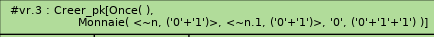
\includegraphics[scale=0.62]{Init.png}
    \caption{\textit{Somme des porte-monnaie à l'intialisation}}
    \label{fig:my_label}
\end{figure}

Sur cette exécution, A remporte la loterie.

\begin{figure}[!h]
    \centering
    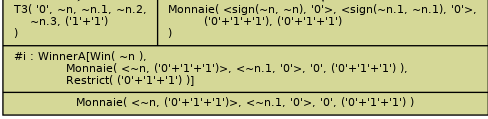
\includegraphics[scale=0.55]{fin.png}
    \caption{\textit{Somme des porte-monnaie après la victoire de A}}
    \label{fig:my_label}
\end{figure}

On remarque que A possède désormais 2 bitcoins, B en possède 0, il n'y a plus d'argent en jeu et la somme d'argent totale est correcte (2 + 0 + 0 = 2). 

La propriété est prouvée automatiquement par Tamarin pour chaque trace. 

\begin{figure}[!h]
    \centering
    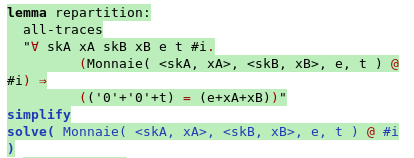
\includegraphics[scale=0.65]{repartition.png}
    \caption{\textit{Propriété pour la répartition correcte de l'argent sur chaque trace prouvée par Tamarin}}
    \label{fig:my_label}
\end{figure}



\section{Conclusion}
Finalement, nous avons réussi à modéliser une exécution du protocole en y intégrant des propriétés simples à modéliser. Ce projet était une véritable découverte du monde de la recherche et nous a permis d'apprendre de nouvelles compétences dans celui-ci. C'était un projet très intéressant sur un sujet d'actualité qui nous a permis d'en apprendre plus sur le monde de la blockchain et des cryptomonnaies. \\

Pour la suite nous avons plusieurs possibilités. Nous avons modélisé des propriétés simples pour nous permettre de vérifier le bon déroulement du protocole. Cependant il y a plusieurs modifications que l'on pourrait faire. Tout d'abord, nous avons modélisé le protocole avec seulement 2 joueurs, le but étant de le modéliser pour N joueurs. Dans ce protocole nous avons aussi défini deux règles WinnerA et WinnerB définissant le gagnant, A ou B. Ces règles ne correspondent pas exactement à celle explicitées dans le protocole de départ. En effet dans la documentation du protocole il est expliqué que le gagnant est défini à partir de la parité des secrets. Ce type de règle étant difficilement implémentable en Tamarin, nous avons décidé de réaliser deux règles définissant que A ou B peuvent gagner. \\

Nous aurions pu également nous intéresser à vérifier des propriétés de \textit{liveness} (la propriété sera vraie après une certaine étape de l'exécution) \cite{vivacite}.
Par exemple, garantir qu'un joueur qui quitte la partie ne peut récupérer son argent qu'avant le premier tour, sinon il perd son argent.


\section{Remerciements}
Nous tenons à remercier M. Steve Kremer et M. Jannik Dreier pour nous avoir proposé ce sujet et nous avoir aidé à modéliser le protocole sur Tamarin. 



\newpage
\bibliographystyle{plain-fr}
\bibliography{bibliography.bib}



\end{document}


